\documentclass{article}

\usepackage[T1, T2A]{fontenc}
\usepackage{fontspec}
\setmainfont{Times New Roman}
\usepackage[utf8]{inputenc}
\usepackage[english, russian]{babel}
\usepackage{geometry}
\usepackage{graphicx}
\usepackage{tocloft}

\graphicspath{ {./img/} }

\renewcommand{\cftsecleader}{\cftdotfill{\cftdotsep}}

\begin{document}

\newgeometry{left=30mm, top=20mm, right=15mm, bottom=20mm, nohead, nofoot}
\begin{titlepage}
\begin{center}
\textbf{Санкт--Петербургский}
\textbf{государственный университет}
\vspace{35mm} \\
\textbf{\textit{\large МИРОШНИЧЕНКО Александр Сергеевич}} \\[8mm]
\textbf{\large Отчет по научно-исследовательской работе}\\[3mm]
\textbf{\textit{\large Улучшение качества изображений с помехами с
использованием генеративных состязательныx сетей}} \\
\vspace{20mm}
Уровень образования: бакалавриат\\
Направление 01.03.02 «Прикладная математика и информатика»\\
Основная образовательная программа СВ.5005.2017
«Прикладная математика, фундаментальная информатика и программирование»\\
Профиль «Исследование и проектирование систем управления\\ и обработки сигналов»\\[30mm]
\begin{flushright}
{Научный руководитель:} \\
доцент, кафедра теории систем управления электрофизической аппаратурой, \\к.ф. - м.н.  Козынченко~Владимир Александрович 
\end{flushright}
\vfill 
{Санкт-Петербург}
\par{2020 г.}
\end{center}
\end{titlepage}
\addtocounter{page}{1}

\tableofcontents

\newpage
\addcontentsline{toc}{section}{Введение}
\section*{Введение}
При съемке фотографии могут возникнуть различные искажения. Например фотография может получится размытой, матрицы фотоаппарата неисправна, или если объектив камеры движется слишком быстро, и не успевает сфокусироваться. В таких случаях можно повторить снимок, но какие-то объекты, которые были засняты в первый раз, уже могут и не появиться в кадре. Иногда фотографию и вовсе нельзя переснять. \\ Встает вопрос о восстановлении качества изображения с помехами.\\
При этом надо понимать, что, конечно, мы не сможем восстановить именно ту фотографию, которая могла получиться, не будь обстоятельств, смазавших кадр. Ведь по сути дела можно представить искажение четкой фотографии как некоторое отображение из множества четких фото в множество размытых. И такое отображение с большой долей вероятности не будет биективным. То есть наверняка существует много различных четких фотографий, которые при обратном отображении в множество размытых дают один и тот же результат.
 \\ Однако можно попытаться сказать, каким мог бы быть один из возможных вариантов четких изображений. \\
Для такой проблемы можно использовать нейронные сети, так как их решают задачу перевода одного тензора данных в другой.

\addcontentsline{toc}{section}{Постановка задачи}
\section*{Постановка задачи}
Реализовать программу, имплементирующую алгоритм улучшения качества размытого изображения при помощи нейронной сети. 

\addcontentsline{toc}{section}{Метод обучения}
\section*{Метод обучения}
Среди существующих видов сетей можно отметить GAN - генеративные состязательные сети. Модели GAN обучаются отображению случайного вектора шума \emph{z} в изображение \emph{y}, G : $\emph{z} \rightarrow \emph{y}$. Условные же GAN учатся преобразованию изображения \emph{x} и случайного вектора шума \emph{z} в изображение \emph{y}, G : $\left\lbrace \emph{x}, \emph{z} \right\rbrace \rightarrow \emph{y}$. 
Генератор G обучается генерировать изображения, которые не может отличить от <<реальных>> дискриминатор D, который, в свою очередь, обучается распознавать <<подделки>> генератора. \\\\
%Размер изображения: $256\times256$ пикселей.
%Язык программирования: Python 3.8
%Библиотеки, используемые для предобработки изображений и написания %нейронной сети: Tensorflow 2.3.0
Целевая функция условной GAN может быть выражена как:
\[\textit{loss}\textsubscript{GAN} = E\textsubscript{\emph{x},\emph{y}}\left[ {\log D\left( \emph{x}, \emph{y} \right) } \right] + E\textsubscript{\emph{x},\emph{z}}\left[ {\log \left( 1 - D\left( \emph{x}, G \left(\emph{x},\emph{z} \right) \right) \right) } \right], \]
где G пытается минимизировать \emph{loss}, в то время как соревнующийся с ним D пытается максимизировать ее. Другими словами G\textsuperscript{*} = $\arg \min_{G} \max_{D} \emph{loss}\textsubscript{GAN}\left( G, D \right)$
\\ В статье о сети pix2pix было проведено исследование, в котором функция L1 в сочетании с традиционной \emph{loss}\textsubscript{GAN} приводила к тому, что работа дискриминатора D не изменялась, а вот генератор G обучался не только обманывать дискриминатор, но и генерировать изображения, близкие к истинным.
\[ L1\left(G\right) = E\textsubscript{\emph{x},\emph{y},\emph{z}}\left[\|\emph{y} - G\left(\emph{x},\emph{z}\right)\|\right]\]
В итоге, наша функция выглядит как:
\[ G\textsuperscript{*} = \arg \min_{G} \max_{D} \emph{loss}\textsubscript{GAN}\left( G, D \right) + \lambda L1\left( G \right) \]
Значение $\lambda=100$, так как именно это значение предлагают авторы вышеупомянутой статьи. \\
Алгоритм обучения представлен на рисунке $\left[ \ref{fig:one_step}\right]$ . Датасет изначально перемешан и разбит на батчи. В данном случае размер батча равен одному. Прогон каждого батча и изменение весов сети обозначены одним шагом обучения.

\begin{figure}[h!]
  \[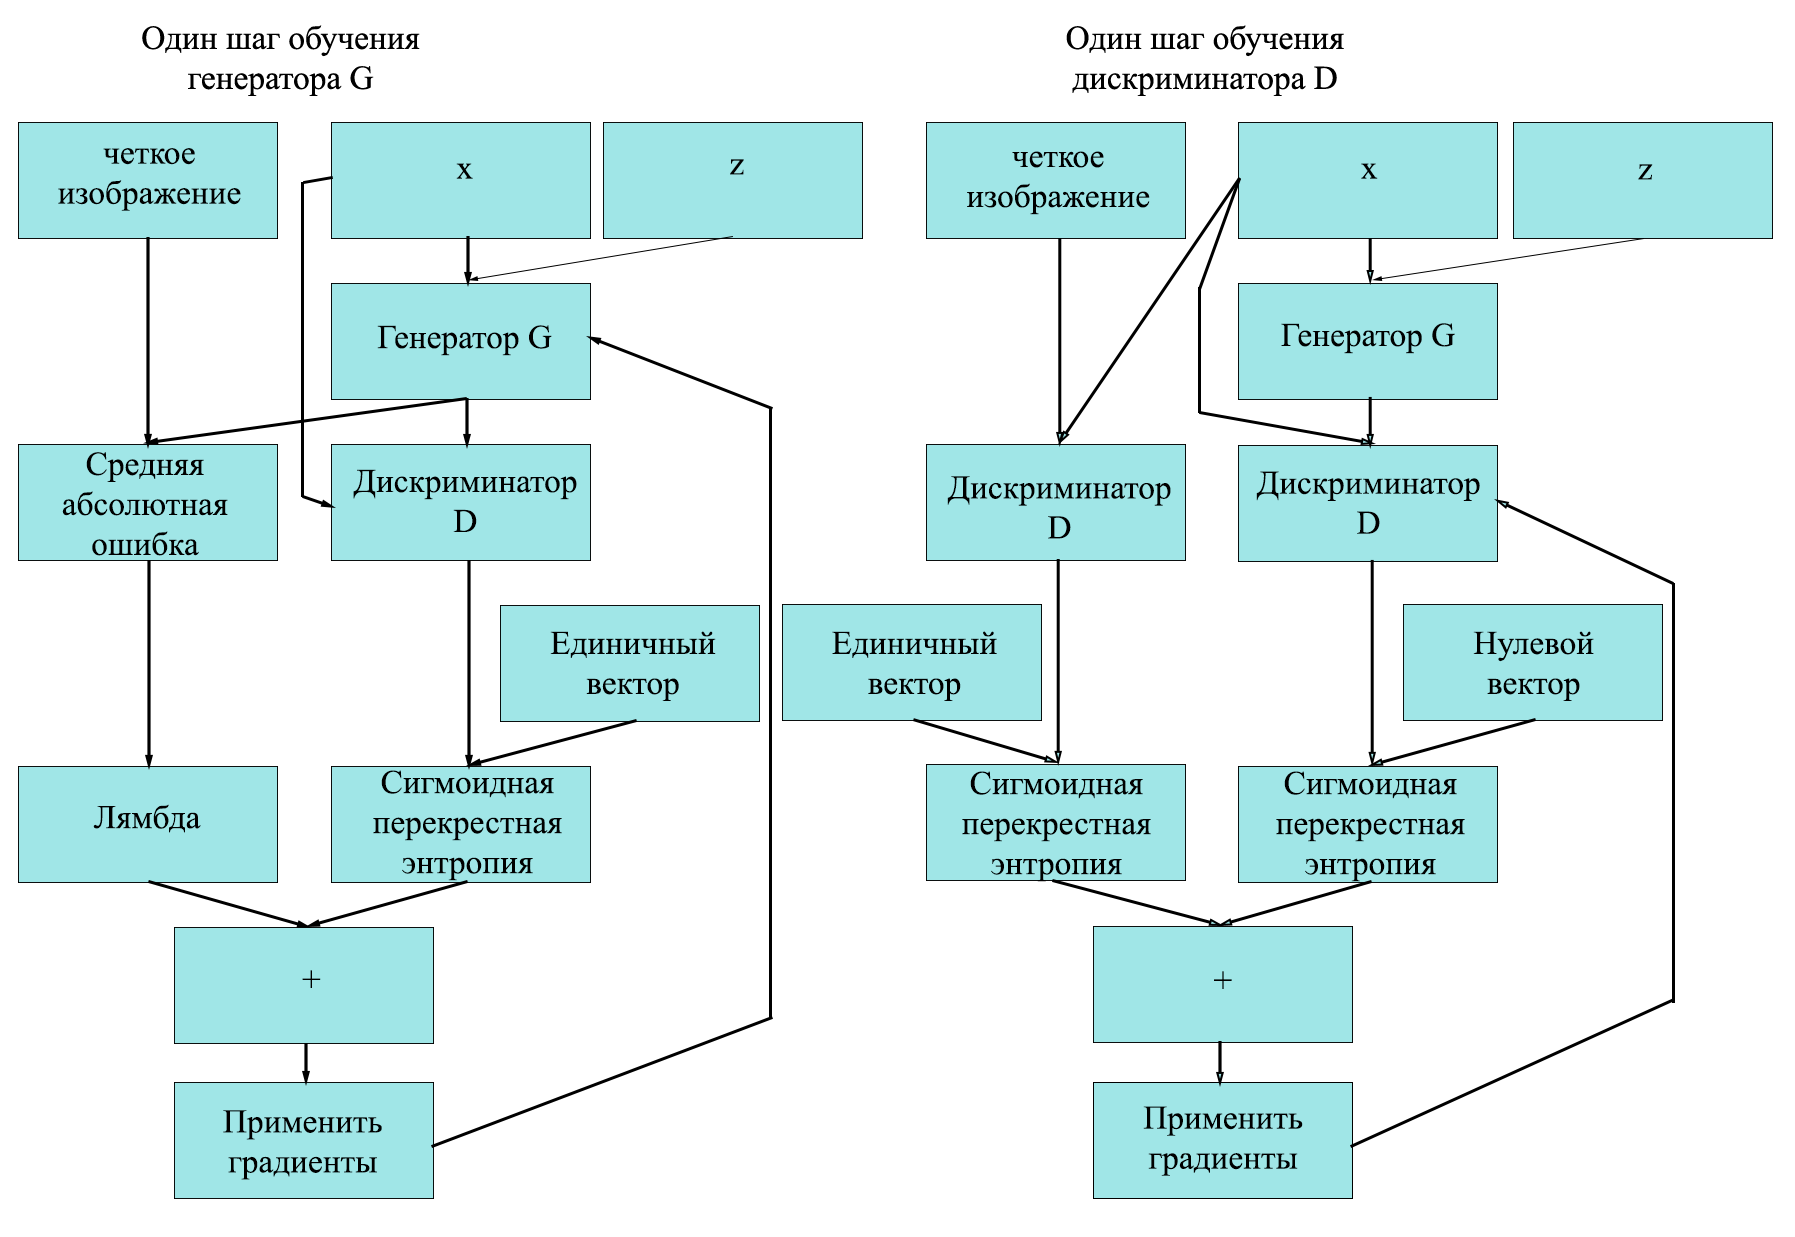
\includegraphics[scale=0.25]{one_step.png}\]
  \caption{Шаг обучения для генератора и дискриминатора}
  \label{fig:one_step}
\end{figure}

\addcontentsline{toc}{section}{Подготовка данных для обучения}
\section*{Подготовка данных для обучения}
Для того, чтобы обучить нейронную сеть, необходимо иметь как размытые изображения \emph{x}, так и четкие изображения \emph{y}. Четкие изображения \emph{y} было решено взять из открытого датасета places365, состоящего из 365 категорий четких фотографий, собранных из интернета. Из этих категорий были выбраны следующие 4: замки, леса, горы и небоскребы. Для тренировочного датасета из каждой категории было выбрано по 250 фотографий, а для тестового - 150. На каждую фотографию был наложен эффект размытия при помощи функции cv2.blur() с ядром $\left( 14, 14 \right)$ из библиотеки OpenCV. Это имитация реальных помех, которые могут произойти при съемке фотографий. Всего получилось 2000 изображений (1000 четких и 1000 размытых) для тренировочного датасета и 1200 изображений (600 четких и 600 размытых) для тестового датасета. Затем эти 2 датасета были переведены в формат numpy массивов с размерностями 1000*2*256*256*3.
После обработки датасеты были загружены на облако Google Drive.


\addcontentsline{toc}{section}{Процесс обучения}
\section*{Процесс обучения}

\addcontentsline{toc}{section}{Анализ полученных результатов}
\section*{Анализ полученных результатов}

\addcontentsline{toc}{section}{Заключение}
\section*{Заключение}

\addcontentsline{toc}{section}{Список литературы}
\section*{Список литературы}

\addcontentsline{toc}{section}{Приложение}
\section*{Приложение}
Ссылка на репозиторий c кодом: 
\restoregeometry
\end{document}
